\chapter{Limits}
\label{Limits_Chapter}

\section{Limit of a sequence}

\section{Limit of a function}

\section{Continuity}

\noindent The concept of continuity is introduced to formalize the intuitive notion of a function without any "`jumps"'. The following graph shows a function that has two such "`jumps"'. 
\begin{center}
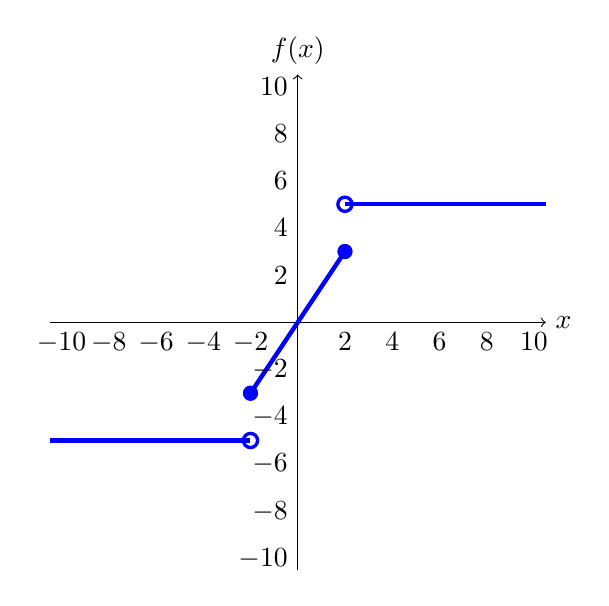
\begin{tikzpicture}[scale=0.3]

	\draw[->]  (0,-10.5)--(0,10.5);
	\draw[->]  (-10.5,0)--(10.5,0);
	\node [right] at (10.5,0) {$x$};
	\node [above] at (0,10.5) {$f(x)$};
	\draw[blue, ultra thick] (-10.5,-5) -- (-2,-5);
	\draw[blue, ultra thick] (2,5) -- (10.5,5);
	\draw[blue, ultra thick] (-2,-3) -- (2,3);
	\draw[blue, very thick](-2, -5) circle (3mm);
	\draw[blue, very thick](2, 5) circle (3mm);
	\filldraw [blue] (-2,-3) circle (3mm);
	\filldraw [blue] (2,3) circle (3mm);
	
 \foreach \x/\xtext in {-10/-10, -8/-8, -6/-6, -4/-4, -2/-2, 0/ , 2/2, 4/4, 6/6, 8/8 , 10/10}
    \draw[shift={(\x,0)}] (0pt,0.3pt) -- (0pt,-0.3pt) node[below] {$\xtext$};

 \foreach \y/\ytext in {-10/-10, -8/-8, -6/-6, -4/-4, -2/-2, 0/ , 2/2, 4/4, 6/6, 8/8 , 10/10}
    \draw[shift={(0,\y)}] (0.3pt,0pt) -- (-0.3pt,-0pt) node[left] {$\ytext$};
	
\end{tikzpicture}
\end{center}
\noindent A function is said to be \textbf{continuous in a point $\mathbf{x}$} if it does not "`jump"' in point $x$. The function above is for instance continuous at $x= 5$. Though it is discontinuous in $x=2$. A function is said to be \textbf{continuous} if it is continuous in all its points. Looking back at the graphs in section (\ref{GraphsExamps}) we notice the hyperbola and the tangent are discontinuous while the other $4$ are continuous.\\

\noindent The formal study of continuity will be left for chapter \ref{Limits_Chapter}. For now we only need to have a vaguer, intuitive idea of what it means for a function to be discontinuous because of what this means for physics. 

%There are several equivalent but seemingly different ways of defining continuity in a point. A first one will be given here. Another one will be discussed after introducing the concept of limits in chapter \ref{Limits_Chapter}.

%\subsection{Continuous using $\epsilon$ and $\delta$}
%
%\noindent We say that a function $f$ is continuous at a point $x_0$ if
%\begin{equation}
%\forall \epsilon \in \mathbb{R}^+_0, \exists \delta \in \mathbb{R}^+_0, \forall x \in \left] x_0 - \delta, x_0 + \delta \right[: f(x) \in \left] f(x_0) - \epsilon, f(x_0)+\epsilon \right[
%\end{equation}

